% Template for ICASSP-2024 paper; to be used with:
%          spconf.sty  - ICASSP/ICIP LaTeX style file, and
%          IEEEbib.bst - IEEE bibliography style file.
% --------------------------------------------------------------------------
\documentclass{article}
\usepackage{spconf,amsmath,graphicx}

\usepackage{geometry}
 \geometry{
 a4paper,
 total={170mm,257mm},
 left=20mm,
 top=20mm,
 }

% header

%% natbib
\usepackage{natbib}
\bibliographystyle{plain}

%% comment
\usepackage{comment}

% no automatic indentation
\usepackage{indentfirst}

% manually indent
\usepackage{xargs} % \newcommandx
\usepackage{calc} % calculation
\newcommandx{\tab}[1][1=1]{\hspace{\fpeval{#1 * 10}pt}}
% \newcommand[number of parameters]{output}
% \newcommandx[number of parameters][parameter index = x]{output}
% use parameter index = x to substitute the default argument
% use #1, #2, ... to get the first, second, ... arguments
% \tab for indentation
% \tab{2} for for indentation twice

% note
\newcommandx{\note}[1]{\textit{\textcolor{red}{#1}}}
\newcommand{\todo}{\note{TODO}}
% \note{TODO}

%% math package
\usepackage{amsfonts}
\usepackage{amsmath}
\usepackage{amssymb}
\usepackage{tikz-cd}
\usepackage{mathtools}
\usepackage{amsthm}

%% operator
\DeclareMathOperator{\tr}{tr}
\DeclareMathOperator{\diag}{diag}
\DeclareMathOperator{\sign}{sign}
\DeclareMathOperator{\grad}{grad}
\DeclareMathOperator{\curl}{curl}
\DeclareMathOperator{\Div}{div}
\DeclareMathOperator{\card}{card}
\DeclareMathOperator{\Span}{span}
\DeclareMathOperator{\real}{Re}
\DeclareMathOperator{\imag}{Im}
\DeclareMathOperator{\supp}{supp}
\DeclareMathOperator{\im}{im}
\DeclareMathOperator{\aut}{Aut}
\DeclareMathOperator{\inn}{Inn}
\DeclareMathOperator{\Char}{char}
\DeclareMathOperator{\Sylow}{Syl}
\DeclareMathOperator{\coker}{coker}
\DeclareMathOperator{\inc}{in}
\DeclareMathOperator{\Sd}{Sd}
\DeclareMathOperator{\Hom}{Hom}
\DeclareMathOperator{\interior}{int}
\DeclareMathOperator{\ob}{ob}
\DeclareMathOperator{\Set}{Set}
\DeclareMathOperator{\Top}{Top}
\DeclareMathOperator{\Meas}{Meas}
\DeclareMathOperator{\Grp}{Grp}
\DeclareMathOperator{\Ab}{Ab}
\DeclareMathOperator{\Ch}{Ch}
\DeclareMathOperator{\Fun}{Fun}
\DeclareMathOperator{\Gr}{Gr}
\DeclareMathOperator{\End}{End}
\DeclareMathOperator{\Ad}{Ad}
\DeclareMathOperator{\ad}{ad}
\DeclareMathOperator{\Bil}{Bil}
\DeclareMathOperator{\Skew}{Skew}
\DeclareMathOperator{\Tor}{Tor}
\DeclareMathOperator{\Ho}{Ho}
\DeclareMathOperator{\RMod}{R-Mod}
\DeclareMathOperator{\Ev}{Ev}
\DeclareMathOperator{\Nat}{Nat}
\DeclareMathOperator{\id}{id}
\DeclareMathOperator{\Var}{Var}
\DeclareMathOperator{\Cov}{Cov}
\DeclareMathOperator{\RV}{RV}
\DeclareMathOperator{\rank}{rank}

%% pair delimiter
\DeclarePairedDelimiter{\abs}{\lvert}{\rvert}
\DeclarePairedDelimiter{\inner}{\langle}{\rangle}
\DeclarePairedDelimiter{\tuple}{(}{)}
\DeclarePairedDelimiter{\bracket}{[}{]}
\DeclarePairedDelimiter{\set}{\{}{\}}
\DeclarePairedDelimiter{\norm}{\lVert}{\rVert}

%% theorems
\newtheorem{axiom}{Axiom}
\newtheorem{definition}{Definition}
\newtheorem{theorem}{Theorem}
\newtheorem{proposition}{Proposition}
\newtheorem{corollary}{Corollary}
\newtheorem{lemma}{Lemma}
\newtheorem{remark}{Remark}
\newtheorem{claim}{Claim}
\newtheorem{problem}{Problem}
\newtheorem{assumption}{Assumption}
\newtheorem{example}{Example}
\newtheorem{exercise}{Exercise}

%% empty set
\let\oldemptyset\emptyset
\let\emptyset\varnothing

\newcommand\eps{\epsilon}

% mathcal symbols
\newcommand\Tau{\mathcal{T}}
\newcommand\Ball{\mathcal{B}}
\newcommand\Sphere{\mathcal{S}}
\newcommand\bigO{\mathcal{O}}
\newcommand\Power{\mathcal{P}}
\newcommand\Str{\mathcal{S}}


% mathbb symbols
\usepackage{mathrsfs}
\newcommand\N{\mathbb{N}}
\newcommand\Z{\mathbb{Z}}
\newcommand\Q{\mathbb{Q}}
\newcommand\R{\mathbb{R}}
\newcommand\C{\mathbb{C}}
\newcommand\F{\mathbb{F}}
\newcommand\T{\mathbb{T}}
\newcommand\Exp{\mathbb{E}}

% mathrsfs symbols
\newcommand\Borel{\mathscr{B}}

% algorithm
\usepackage{algorithm}
\usepackage{algpseudocode}

% longproof
\newenvironment{longproof}[1][\proofname]{%
  \begin{proof}[#1]$ $\par\nobreak\ignorespaces
}{%
  \end{proof}
}


% for (i) enumerate
% \begin{enumerate}[label=(\roman*)]
%   \item First item
%   \item Second item
%   \item Third item
% \end{enumerate}
\usepackage{enumitem}

% insert url by \url{}
\usepackage{hyperref}

% margin
\usepackage{geometry}
\geometry{
a4paper,
total={190mm,257mm},
left=10mm,
top=20mm,
}



% Example definitions.
% --------------------
\def\x{{\mathbf x}}
\def\L{{\cal L}}

% Title.
% ------
\title{
Streaming Spectral Clustering with Krylov Block Iteration Technical Document
}
%
% Single address.
% ---------------
\name{Nguyen Ngoc Khanh, Teh Kah Kuan, Jayakrishnan Melur Madhathil, Sun Hanwu, Tran Huy Dat}
\address{}





%
% For example:
% ------------
%\address{School\\
%	Department\\
%	Address}
%
% Two addresses (uncomment and modify for two-address case).
% ----------------------------------------------------------
%\twoauthors
%  {A. Author-one, B. Author-two\sthanks{Thanks to XYZ agency for funding.}}
%	{School A-B\\
%	Department A-B\\
%	Address A-B}
%  {C. Author-three, D. Author-four\sthanks{The fourth author performed the work
%	while at ...}}
%	{School C-D\\
%	Department C-D\\
%	Address C-D}
%
\begin{document}
%\ninept
%

\maketitle


\section{Problem Statement and Method Summary}
The problem is the real-time implementation of spectral clustering algorithm of high dimensional embedding features which achieves top performance for the task of speaker diarisation but is hard to implement in a streaming mode as requiring full matrix operations on Laplacian kernel matrix. This TD proposes a novel iterative way to conduct that operations by applying a trick in cosine similarity kernel decomposition, making it to a tractable form expression to the mathematical problem, to enable the implementation in an iterative streaming fashion and also possible to further adoptions of Krylov low-rank approximation making it even faster and more accurate.

\section{Spectral Clustering}
Let $X \in \R^{n \times m}$ be the data matrix and a similarity function $k: \R^m \times \R^m \to [0, \infty)$. \textit{Spectral Clustering} constructs the similarity matrix $W \in \R^{n \times n}$ where each entry $W_{i j} = k(x_i, x_j)$. The Laplacian matrix is then calculated as $\mathcal{L} = I - D^{-1/2} W D^{-1/2}$. Based on \textit{Spectral Graph Theory}, the first $K$ eigenvectors of $\mathcal{L}$ well represents data under the similarity function $k$. \textit{K-means} is then used to form clusters from eigenvectors of $\mathcal{L}$.

\section{Streaming Spectral Clustering with Block Krylov Iteration}

Figure \ref{fig:spectral} shows the difference between \textit{Streaming Spectral Clustering} and \textit{Offline Spectral Clustering}.

\begin{figure}[htb]
    \begin{minipage}[b]{1.0\linewidth}
    \centering
    \centerline{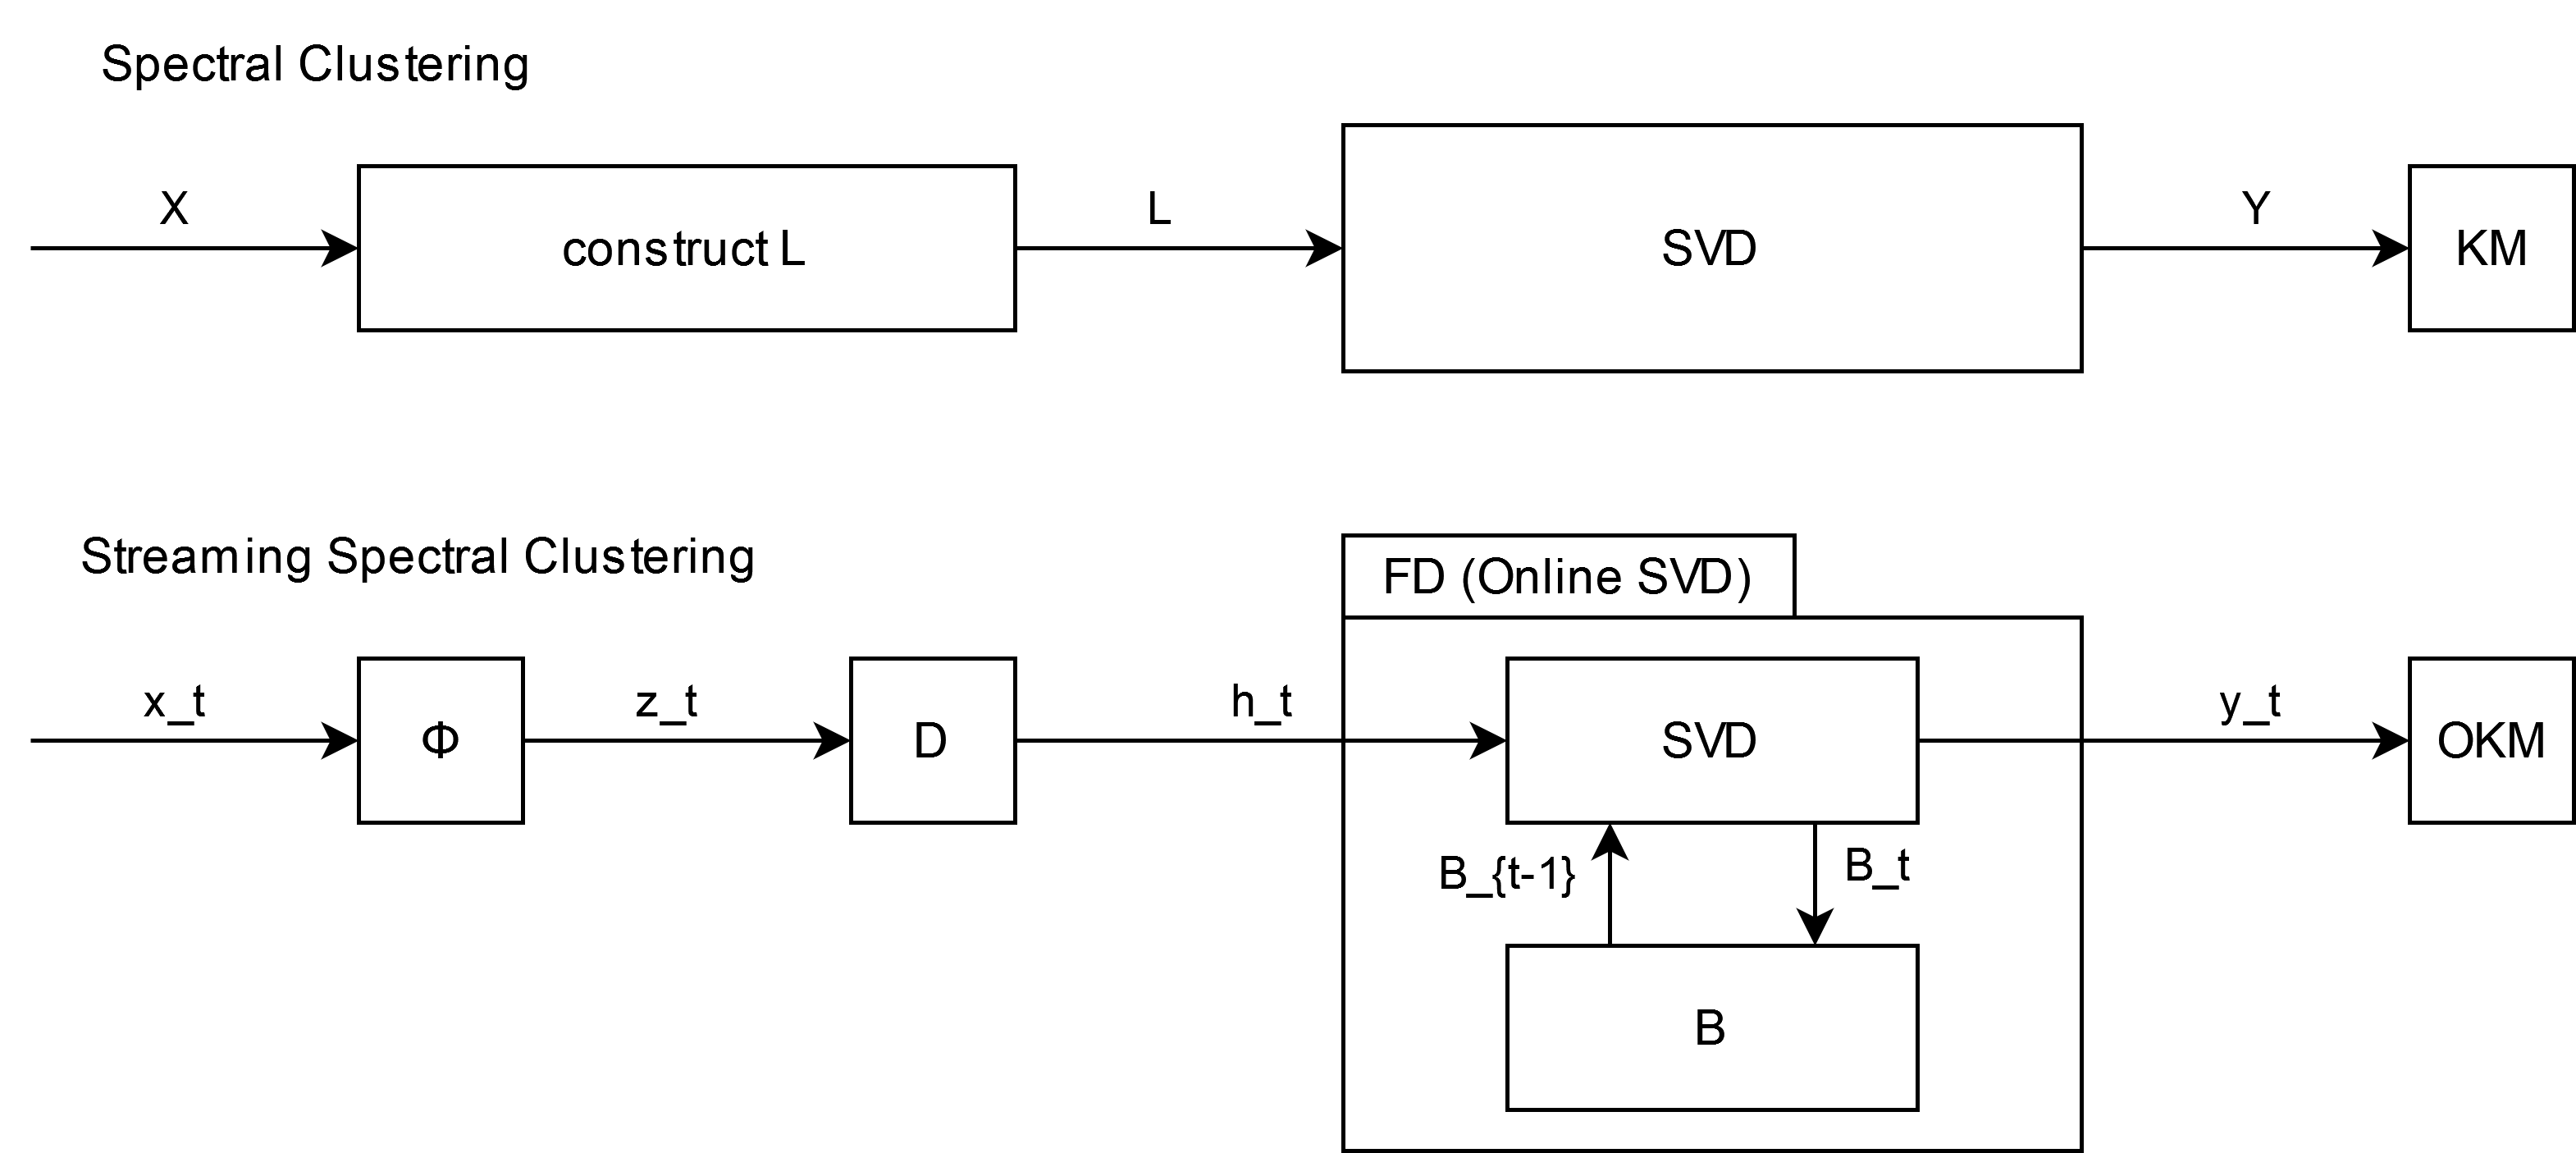
\includegraphics[width=8.5cm]{assets/ssc_diagram.png}}
    %\vspace{2.0cm}
    \end{minipage}
\caption{Speaker Diarization Pipeline}
\label{fig:spectral}
\end{figure}

In the online setup, let $X \in \R^{n \times m}$ be the data matrix where each row $x_t \in \R^{m}, t=1, 2, ..., n$ is recorded sequentially and a similarity function $k: \R^m \times \R^m \to [0, \infty)$ that is also a kernel. A neat update of the Cholesky decomposition of the Laplacian matrix is presented below.

\subsection{Kernel mapping function ($\phi$)}

Let the similarity function be the cosine function. 
$$
    k(x, y) = \frac{\langle x, y\rangle}{||x||.||y||}
$$
The kernel mapping function $\phi$ transforms each data point $x_t \in \R^m$ into $z_t \in \R^d$ such that $\langle z_i, z_j \rangle = k(x_i, x_j)$. For cosine, the kernel mapping function is
$$
    z_t = \phi(x_t) = \left(1, \frac{x_t^{(1)}}{||x_t||}, \frac{x_t^{(2)}}{||x_t||}, ..., \frac{x_t^{(m)}}{||x_t||}\right) \in \R^{m+1}
$$

\subsection{Degree Matrix Approximation (D)}

After that, normalizing $z_t$ according to the approximated degree matrix as 
$$
    h_t = D(z_t) \approx \frac{z_t}{\sqrt{\langle z_t, c_t \rangle}}
$$
where $c_t = (\sum_{j=1}^t z_j) / ||\sum_{j=1}^t z_j||$. That yields  rows of a matrix $H = (h_1, h_2, ..., h_n)$. The left singular vectors of $H$ coincide with the eigen vectors of the normalized Laplacian $\mathcal{L}$, which enables us to calculate eigenvectors of $\mathcal{L}$ in an online manner by calculating singular vectors of $H$ sequentially.

\subsection{Frequent Direction with Block Krylov Iteration (FD\_BKI)}

FD\_BKI (Algorithm \ref{alg:fd_bki}) is an extension of FD that is used to extract left singular vectors of $H$ sequentially. FD maintains a compression of the stream of data at time $t-1$ by a sketch matrix $B_{t-1} \in \R^{l \times d}$. When a new data point $h_t$ arrives, SVD algorithm is then used to extract the embedding of the $h_t$ sequentially. FD\_BKI adds an additional step (4-6) that both denoises and compresses the input $h_t$ based on the theory of Krylov subspace and Chebyshev polynomials.

\subsection{Online K-means (OKM)}

Similar to \textit{Offline Spectral Clustering}, \textit{Online K-means} is used to form clusters from singular vectors of $H$ in an online manner.


\begin{algorithm}
\caption{BKI \cite{musco2015randomized}}\label{alg:bki}
\begin{algorithmic}[1]
\Require $A \in \R^{n \times d}$, error $\epsilon > 0$, sketch size $l \leq n, d$
\Ensure $Z \in \R^{n \times l}$, $P \in \R^{l \times d}$
\State $q \gets \Theta(\frac{\log d}{\sqrt{\epsilon}})$, $\Pi \sim \mathcal{N}(0, 1)^{d \times l}$
\State $K \gets [A\Pi, (AA^T) A\Pi, ..., (AA^T)^{q-1} A\Pi] \in \R^{n \times lq}$
\State Orthonormalize columns of $K$ to obtain $Q \in \R^{n \times lq}$
\State Set $U_l \in \R^{lq \times l}$ to be the top-$l$ left singular vectors of $Q^T A$
\State $Z \gets Q U_l$, $P \gets Z^T A$
\end{algorithmic}
\end{algorithm}

\begin{algorithm}
\caption{FD \cite{yoo2016streaming} and FD\_BKI}\label{alg:fd_bki}
\begin{algorithmic}[1]
\Require $H = \{P_t \in \R^{b \times d} \}$, error $\epsilon > 0$, sketch size $l \ll d$, batch size $b$, output dimension $k \leq l$
\Ensure $Y = \{U_t \in \R^{b \times k} \}$, $V_t$

\State $B \gets \text{empty matrix} \in \R^{0 \times d}$

\While{stream $H$ is not empty}
    \State Read $b$ rows from $H$ to obtain $P_t \in \R^{b \times d}$
    \If{BKI is specified to use and $b > l$}
        \State $P_t \gets \text{BKI}(P_t, \epsilon, l)$ 
    \EndIf
    \State Append $P_t$ into $B$
    % \State  $U_t, V_t \gets \text{FD\_EXTRACT}(B, P_t)$
    \State $U, \Sigma, V \gets \text{SVD}(B)$
    \State $V_t \gets V_{[k]}, U_t \gets P_t V_{[k]} \Sigma_{[k]}^{-1}$
    \If{number of rows of $B \geq 2l$}
        % \State $B \gets \text{FD\_PRUNE}(B)$
        \State $\Bar{\Sigma} \gets \diag \left( \sqrt{\max \{0, \sigma^2 - \sigma_l^2\}}\right)$
        \State $B \gets \Bar{\Sigma}_{[l]} V_{[l]}^T$
    \EndIf
\EndWhile

\end{algorithmic}
\end{algorithm}
\chapter{Experiment}
Our initialization for table assignment was chosen such at each customer is at a separate table at the beginning. Louvain method \cite{blondel2008fast} was used in MCLA algorithm due to its low time complexity.
\section{Synthetic Networks}

\subsection{Setup}

In this section, the performance of proposed method is demonstrated using synthetic network as described below:

\begin{algorithm}[H]
\label{alg:powerlaw}
\caption{Power-Law clustering generator}
\textbf{Input:}\\
    $\gamma$: gamma constant \\
    $K$: number of clusters\\

\textbf{Output:}\\
    $size$: relative sizes of clusters distributed according to density $f(x) \propto x^{-\gamma}$\\
    
\begin{algorithmic}

\State $size = \{\frac{k - 0.5}{K}\}_{k=1}^{K}$

\State $size = size^\frac{1}{1 - \gamma}$ \Comment{Element-wise operation}

\State $size = \frac{size}{size.sum()}$ \Comment{Element-wise operation}

\end{algorithmic}
\end{algorithm}

Stochastic Block Model is used to generate the networks with power-law cluster sizes, average degree and intra-cluster edge probability over inter-cluster edge probability $p_{in} / p_{out} = 10$.

We performed grid search over the set of parameters as follow: Number of vertices $|V| \in \{500, 1000, 1500, 2000\}$, average degree $avgdeg \in \{10, 20, 30, 40, 50\}$, scale parameter $s \in \{1000, 2000, ..., 29000\}$

The same node embedding from \emph{Deepwalk} was used for different scale parameter. We fixed these parameters: $\gamma = 2.5$, embedding dimension $d=50$, walks per vertex $\gamma = 2|E|/|V|$, context size $c = 5$, walk length $l = 3c$, receptive field hop $h=1$, \emph{Deepwalk} epochs = 10 and \emph{ddCRP} epochs = 10 for each run. We took only the last 5 iterations from \emph{ddCRP} as the set of stable states.

We compared two versions: initialized Kmeans using ddCRP and MCLA \textbf{ddcrp-mcla} and initialized Kmeans "k-means++" \textbf{kmeans++} with 10 times of initialization which is builtin within sklearn library.

\subsection{Results}
\subsubsection{Modularity}

\begin{figure}
    \centering
    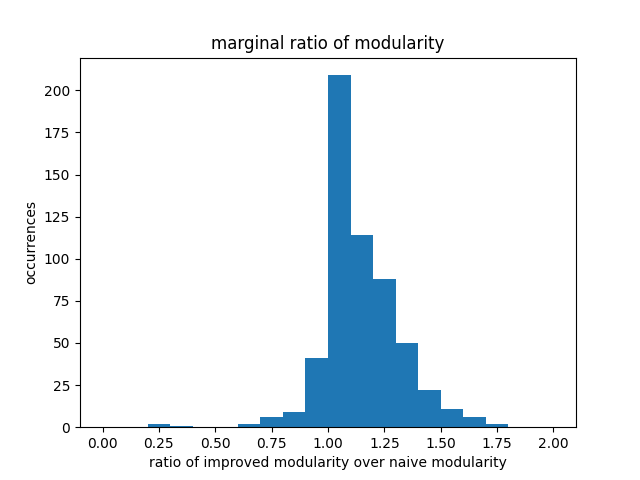
\includegraphics[width=0.8\textwidth]{report/assets/results/ratio.png}
    \caption{Distribution of ratio $\frac{\text{modularity(ddcrp-mcla)}}{\text{modularity(kmeans++)}}$}
    \label{fig:ratio}
\end{figure}


Modularity of each algorithm was evaluated for each setup. Figure \ref{fig:ratio} represent the distribution of the ratio $\frac{\text{modularity(ddcrp-mcla)}}{\text{modularity(kmeans++)}}$. The figure reflects the superior performance of \textbf{ddcrp-mcla} initialization for kmeans as compare to \textbf{kmeans++}. On average, \textbf{ddcrp-mcla} performs better than \textbf{kmeans++} by 14.1\% with a standard deviation of 17.5\%.

Figure \ref{fig:modularity10}, \ref{fig:modularity20}, \ref{fig:modularity30}, \ref{fig:modularity40}, and \ref{fig:modularity50} show that the modularity obtained by \textbf{ddcrp-mcla} always better than \textbf{kmeans++} on all different predicted number of clusters even if the estimation diverges from the true number of clusters (50).

\begin{figure}
    \centering
    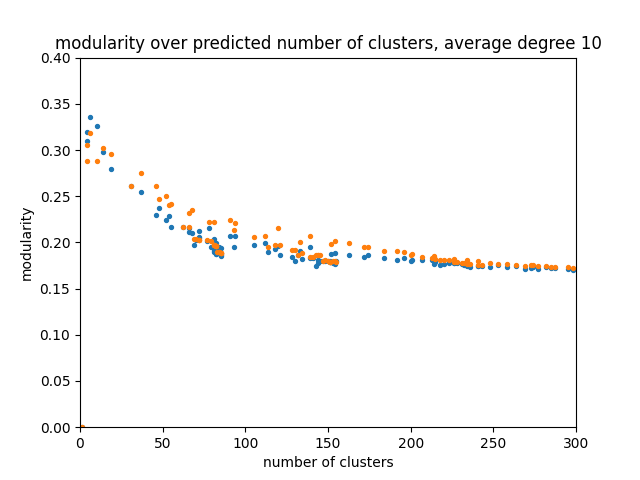
\includegraphics[width=0.8\textwidth]{report/assets/results/modularity10.png}
    \caption{Modularity w.r.t predicted number of clusters for average degree 10 (\textbf{ddcrp-mcla}: orange, \textbf{kmeans++}: blue)}
    \label{fig:modularity10}
\end{figure}

\begin{figure}
    \centering
    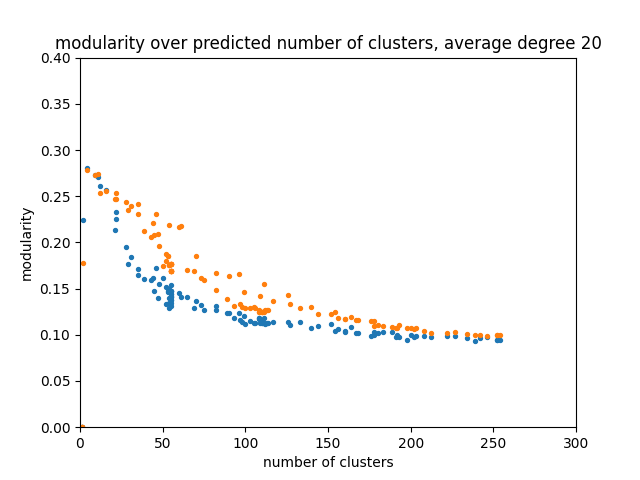
\includegraphics[width=0.8\textwidth]{report/assets/results/modularity20.png}
    \caption{Modularity w.r.t predicted number of clusters for average degree 20 (\textbf{ddcrp-mcla}: orange, \textbf{kmeans++}: blue)}
    \label{fig:modularity20}
\end{figure}

\begin{figure}
    \centering
    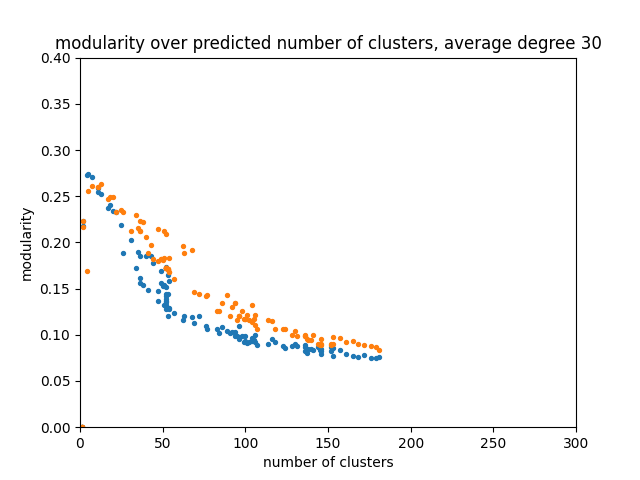
\includegraphics[width=0.8\textwidth]{report/assets/results/modularity30.png}
    \caption{Modularity w.r.t predicted number of clusters for average degree 30 (\textbf{ddcrp-mcla}: orange, \textbf{kmeans++}: blue)}
    \label{fig:modularity30}
\end{figure}

\begin{figure}
    \centering
    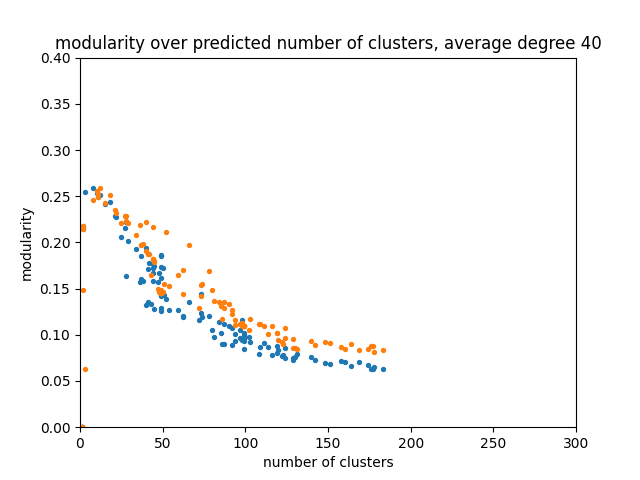
\includegraphics[width=0.8\textwidth]{report/assets/results/modularity40.png}
    \caption{Modularity w.r.t predicted number of clusters for average degree 40 (\textbf{ddcrp-mcla}: orange, \textbf{kmeans++}: blue)}
    \label{fig:modularity40}
\end{figure}

\begin{figure}
    \centering
    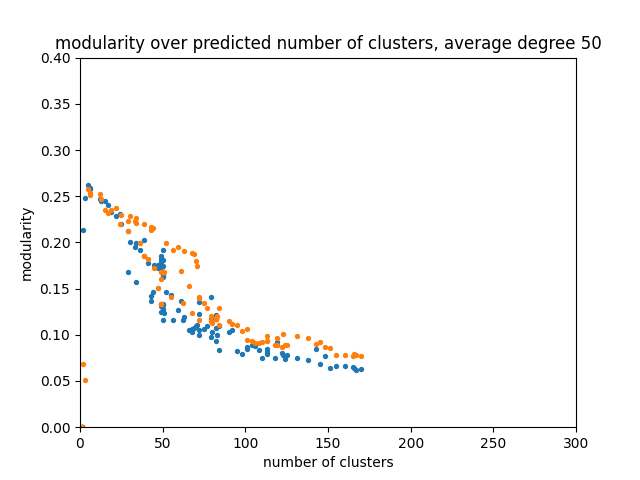
\includegraphics[width=0.8\textwidth]{report/assets/results/modularity50.png}
    \caption{Modularity w.r.t predicted number of clusters for average degree 50 (\textbf{ddcrp-mcla}: orange, \textbf{kmeans++}: blue)}
    \label{fig:modularity50}
\end{figure}

The ratio $\frac{\text{modularity(ddcrp-mcla)}}{\text{modularity(kmeans++)}}$ depends on its predicted number of clusters as shown in figure \ref{fig:ratio_cluster}. The ratio appears to achieve its best performance at the predicted number of clusters between 50 and 100 where the actual number of clusters is 50.

\begin{figure}
    \centering
    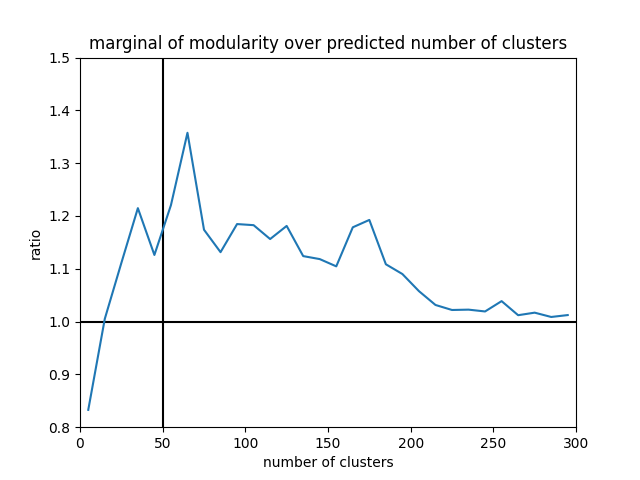
\includegraphics[width=0.8\textwidth]{report/assets/results/ratio_cluster.png}
    \caption{ratio $\frac{\text{modularity(ddcrp-mcla)}}{\text{modularity(kmeans++)}}$ over predicted number of clusters}
    \label{fig:ratio_cluster}
\end{figure}

\section{Real Networks}

\subsection{Setup}

In this experiment, we used the dataset at \cite{paranjape2017motifs}. The temporal network consists of 986 nodes and 332334 temporal edges in the time span of 803 days. We firstly sorted the temporal edges by its timestamp. Then we splitted the set of temporal edges into 1000 equal folds where each fold has roughly 332 edges. We set the window size of 10 folds. After each iteration, we slided the window by 1 fold. We then took the two edge timestamps of the window and filtered all the temporal edges between these timestamps as the set of edges for the graph snapshot.

Similar to the previous experiment, we set embedding dimension $d=50$, walks per vertex $\gamma = 2|E|/|V|$, context size $c = 5$, walk length $l = 3c$, \emph{Deepwalk} epochs = 10 and \emph{ddCRP} epochs = 10 for each run. We took only the last 5 iterations from \emph{ddCRP} as the set of stable states.

We performed grid search over the set of parameters as follow. Receptive field hop $h \in \{1, 2\}$, scale parameter $s \in \{1000, 2000, ..., 8000\}$

\subsection{Results}
\subsubsection{Modularity}
Figure \ref{fig:ratio_cluster_real} shows the ratio between $\frac{\text{modularity(ddcrp-mcla)}}{\text{modularity(kmeans++)}}$ over different predicted number of clusters. If we limit the predicted number of clusters to be greater than 60, the \textbf{ddcrp-mcla} method performs better than \textbf{kmeans++} by 4.4\% with a standard deviation of 5.6\%.

\begin{figure}
    \centering
    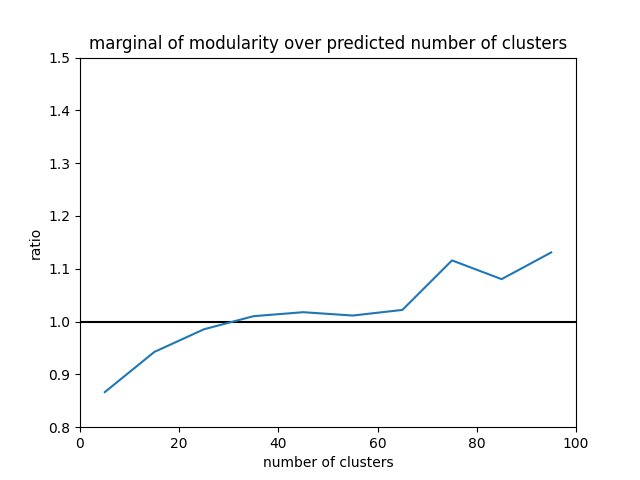
\includegraphics[width=0.8\textwidth]{report/assets/results/ratio_cluster_real.png}
    \caption{ratio $\frac{\text{modularity(ddcrp-mcla)}}{\text{modularity(kmeans++)}}$ over predicted number of clusters}
    \label{fig:ratio_cluster_real}
\end{figure}

\subsubsection{Clustering Evolution}

Our \emph{MCLA} algorithm is capable to produce some useful response from the evolution of clustering. Noted that, these results are completely automated. Textbox \ref{textbox:message}.

\fbox{\begin{minipage}{15em}
message type: join

	9 nodes remained
	
	3 nodes joined
	
	0 nodes left
	
message type: old

	2 nodes remained
	
	0 nodes joined
	
	0 nodes left
	
message type: old

	0 nodes remained
	
	25 nodes joined
	
	7 nodes left
	
message type: old

	3 nodes remained
	
	0 nodes joined
	
	0 nodes left
	
message type: join

	418 nodes remained
	
	0 nodes joined
	
	153 nodes left
	
	...
\label{textbox:message}
\end{minipage}}




% To start a new column (but not a new page) and help balance the last-page
% column length use \vfill\pagebreak.
% -------------------------------------------------------------------------
%\vfill
%\pagebreak


\vfill\pagebreak


% References should be produced using the bibtex program from suitable
% BiBTeX files (here: strings, refs, manuals). The IEEEbib.bst bibliography
% style file from IEEE produces unsorted bibliography list.
% -------------------------------------------------------------------------


\bibliographystyle{IEEEbib}
\bibliography{references}



\end{document}
